\chapter{Introduction to R and RStudio}

Various statistical and programming software environments are used in data science, including R, Python, SAS, C++, SPSS, and many others. Each has strengths and weaknesses, and often two or more are used in a single project. This book focuses on R, for several reasons. One important reason is that R is free. Another is that R is one of, if not the, most widely used software environments in data science. A third is that R is under constant and open development by a diverse and expert core group, and that R also includes an incredible variety of contributed packages. A fourth reason is that a new user can (relatively) quickly gain enough skills to obtain, manage, and analyze data in R. 

Several enhanced interfaces for R have been developed. Generally such interfaces are referred to as an integrated development environment (IDE) and are programs to facilitate software development. At minimum, an IDE typically consists of a source code editor and build automation tools. We will use the RStudio IDE, which according to its developers ``is a powerful productive user interface for R.''\footnote{http://www.rstudio.com/} RStudio is widely used, its use is increasing in the R community, and it makes learning to use R a bit simpler. Although we will use RStudio, most of what is presented in this book can be accomplished in R (without an added interface) with few or no changes. 

\section{Obtaining and installing R}
It is simple to install R on computers running Microsoft Windows, OS X (Mac), and Linux. For other operating systems users can compile the source code directly.\footnote{Windows, OS X, and Linux users also can compile the source code directly, but for most it is a better idea to install R from already compiled binary distributions.}
Here is a step-by-step guide to installing R for Microsoft Windows.\footnote{New versions of R are released regularly, so the version number in Step~\ref{STEP:VERSION} might be different from what is listed below.} OS X and Linux users would follow similar steps.
\begin{enumerate}
\item Go to \url{http://www.r-project.org/}
\item Click on the \texttt{CRAN} link on the left side of the page
\item Choose one of the mirrors.\footnote{The \url{http://cran.rstudio.com/} mirror is usually fast. Otherwise choose a mirror in Michigan.}
\item Click on \texttt{Download R for Windows}
\item Click on \texttt{base}
\item \label{STEP:VERSION} Click on \texttt{Download R 3.3.3 for Windows}
\item Install R as you would install any other Windows program
\end{enumerate}
\section{Obtaining and installing RStudio}

You must install R prior to installing RStudio. RStudio is also simple to install:
\begin{enumerate}
\item Go to \url{http://www.rstudio.com}
\item Click on the link \texttt{RStudio} under the \texttt{Products} tab, then select the \texttt{Desktop} option
\item Click on the \texttt{Desktop} link
\item Choose the \texttt{DOWNLOAD RSTUDIO DESKTOP} link in the \texttt{Open Source Edition} column
\item On the ensuing page, click on the \texttt{Installer} version for your operating system, and once downloaded, install as you would any program
\end{enumerate}

\section{RStudio Server}
An alternative to installing R and RStudio on your computer is to use RStudio Server. RStudio Server is a web browser based interface to a current version of R and RStudio. Through this course, you have access to RStudio Server and disk space to store your work and exercises. The only requirements are that you have a fast and reliable internet connection. You can access your RStudio Server account at \url{http://rstudio.itservices.msu.edu}. Your username is your MSU NetID, and your password is your first name appended to your MSU student ID number (APID), with both the ``A'' starting your PID and the first letter in your first name capitalized. For example, my username would be \emph{finleya} and my password \emph{A8675309Andrew}\footnote{Not surprisingly, this is not really my MSU APID.}.

This is not a great password because your APID is not private. So, when you first log in, you must change your password to something much more cryptic. Here are the steps to change your password after logging in:
\begin{enumerate}
\item Open the \texttt{tools} menu at the top
\item Click \texttt{Shell...} and a new window will open
\item Type ``passwd'' in the shell window (without the quotes) and press enter
\item Enter current password and press enter
\item Enter new password and press enter
\item Enter your new password again to confirm and press enter
\item You can close the window after you get a confirmation that your password was updated (i.e., the message ``passwd: all authentication tokens updated successfully.'')
\end{enumerate}
    
There are advantages and disadvantages to using RStudio Server versus a local install of RStudio on your computer. 

\textbf{Some advantages}:
\begin{itemize}
\item You don't need to install RStudio on your computer
\item You don't need to install the R packages used in the course (we've already installed them on the server before the course ends)
\item You have plenty of remote (on the cloud) space to save your exercises and related work
\item You can access the RStudio Server and course work using any computer with fast and reliable internet
\end{itemize}

\textbf{Some disadvantages}: 
\begin{itemize}
\item You don't learn firsthand the steps needed to install RStudio and necessary R packages on a computer
\item Your access to RStudio Server and course work disappears at the end of the semester (although you can always download a copy of your work)
\item It's a bit cumbersome to move files to and from the server for each exercise
\item You can't do your work offline (you must be connected)
\item The server might be slow if there are many users logged in
\end{itemize}

There are some minor difference between RStudio Server and RStudio that are highlighted in the video at the end of this chapter. Examples given in the remainder of this chapter assume you are using a local install of RStudio (but are applicable to a RStudio Server session).

You are free to use RStudio Server and/or a local install of R/RStudio for this course.

\section{Using R and RStudio}
Start RStudio as you would any other program in your operating system. For example under Microsoft Windows it can be run via the Start Menu or by double clicking on the shortcut on the desktop, if a shortcut was created in the installation process.  A (rather small) view of RStudio is displayed in Figure~\ref{FIG:RSTUDIO}.
\begin{figure}[htbp]
\includegraphics*[width=6.5in]{chapter2/RStudio.png}
\caption{The RStudio IDE.}
\label{FIG:RSTUDIO}
\end{figure}

Initially the RStudio window contains three smaller windows. For now our main focus will be the large window on the left, the \verb+Console+ window. R statements are typed in this window. The next few sections give simple examples of the use of R. In these sections we will focus on small and non-complex data sets, but of course later in the book we will work with much larger and more complex sets of data.  Read these sections at your computer with R running, and enter the R commands there to get comfortable using the R console window and RStudio.

\subsection{R as a calculator}
R can be used as a calculator. Note that \verb+#+ is the comment character in R, so R ignores everything following this character. Also, you will see that R prints \texttt{[1]} before the results of each command. Ignore this for now. Soon its relevance will be explained. The command prompt  in R is the greater than sign \verb+>+. 
\begin{Schunk}
\begin{Sinput}
> 34+20*sqrt(100)  ## +,-,*,/ have the expected meanings
\end{Sinput}
\begin{Soutput}
[1] 234
\end{Soutput}
\begin{Sinput}
> exp(2)  ##The exponential function
\end{Sinput}
\begin{Soutput}
[1] 7.389056
\end{Soutput}
\begin{Sinput}
> log10(100)  ##Base 10 logarithm
\end{Sinput}
\begin{Soutput}
[1] 2
\end{Soutput}
\begin{Sinput}
> log(100)  ##Base e logarithm
\end{Sinput}
\begin{Soutput}
[1] 4.60517
\end{Soutput}
\begin{Sinput}
> 10^log10(55)
\end{Sinput}
\begin{Soutput}
[1] 55
\end{Soutput}
\end{Schunk}

Most functions in R can be applied to vector arguments rather than operating on a single argument at a time. A vector is a data structure that contains elements of the same data type (i.e. integers).

\begin{Schunk}
\begin{Sinput}
> 1:25 ##The integers from 1 to 25
\end{Sinput}
\begin{Soutput}
 [1]  1  2  3  4  5  6  7  8  9 10 11 12 13 14 15 16 17 18 19 20 21 22 23 24 25
\end{Soutput}
\begin{Sinput}
> log(1:25) ##The base e logarithm of these integers
\end{Sinput}
\begin{Soutput}
 [1] 0.0000000 0.6931472 1.0986123 1.3862944 1.6094379 1.7917595 1.9459101
 [8] 2.0794415 2.1972246 2.3025851 2.3978953 2.4849066 2.5649494 2.6390573
[15] 2.7080502 2.7725887 2.8332133 2.8903718 2.9444390 2.9957323 3.0445224
[22] 3.0910425 3.1354942 3.1780538 3.2188758
\end{Soutput}
\begin{Sinput}
> 1:25*1:25 ##What will this produce?
\end{Sinput}
\begin{Soutput}
 [1]   1   4   9  16  25  36  49  64  81 100 121 144 169 196 225 256 289 324 361
[20] 400 441 484 529 576 625
\end{Soutput}
\begin{Sinput}
> 1:25*1:5 ##What about this?
\end{Sinput}
\begin{Soutput}
 [1]   1   4   9  16  25   6  14  24  36  50  11  24  39  56  75  16  34  54  76
[20] 100  21  44  69  96 125
\end{Soutput}
\begin{Sinput}
> seq(from=0, to=1, by=0.1) ##A sequence of numbers from 0 to 1
\end{Sinput}
\begin{Soutput}
 [1] 0.0 0.1 0.2 0.3 0.4 0.5 0.6 0.7 0.8 0.9 1.0
\end{Soutput}
\begin{Sinput}
> exp(seq(from=0, to=1, by=0.1)) ##What will this produce?
\end{Sinput}
\begin{Soutput}
 [1] 1.000000 1.105171 1.221403 1.349859 1.491825 1.648721 1.822119 2.013753
 [9] 2.225541 2.459603 2.718282
\end{Soutput}
\end{Schunk}

Now the mysterious square bracketed numbers appearing next to the output make sense. R puts the position of the beginning value on a line in square brackets before the line of output. For example if the output has 40 values, and 15 values appear on each line, then the first line will have \verb+[1]+ at the left, the second line will have \verb+[16]+ to the left, and the third line will have \verb+[31]+ to the left.

\subsection{Basic descriptive statistics and graphics in R}\label{sec:dec}
Of course it is easy to compute basic descriptive statistics and to produce standard graphical representations of data. First we create variables with horsepower and miles per gallon. and names for 15 cars.\footnote{These are from a relatively old data set, with 1974 model cars.} In this case with a small data set we enter the data ``by hand'' using the \verb+c()+ function, which concatenates its arguments into a vector. For larger data sets we will clearly want an alternative. Note that character values are surrounded by quotation marks.

A style note: R has two widely used methods of assignment: the left arrow, which consists of a less than sign followed immediately by a dash: \verb+<-+ and the equals sign: \verb+=+. Much ink has been used debating the relative merits of the two methods, and their subtle differences. Many leading R style guides (e.g., the Google style guide at \url{https://google.github.io/styleguide/Rguide.xml} and the Bioconductor style guide at \url{http://www.bioconductor.org/developers/how-to/coding-style/}) recommend the left arrow \verb+<-+ as an assignment operator, and it will be used below. 

Also you will see that if a command has not been completed but the ENTER key is pressed, the command prompt changes to a \verb-+- sign.
\begin{Schunk}
\begin{Sinput}
> car.hp <- c(110, 110, 93, 110, 175, 105, 245, 62, 95, 123, 
+ 123, 180, 180, 180, 205)
> car.mpg <- c(21.0, 21.0, 22.8, 21.4, 18.7, 18.1, 14.3, 24.4, 22.8, 
+              19.2, 17.8, 16.4, 17.3, 15.2, 10.4)
> car.name <- c("Mazda RX4", "Mazda RX4 Wag", "Datsun 710", 
+               "Hornet 4 Drive", "Hornet Sportabout", "Valiant", 
+               "Duster 360", "Merc 240D", "Merc 230", "Merc 280", 
+               "Merc 280C", "Merc 450SE", "Merc 450SL", 
+               "Merc 450SLC", "Cadillac Fleetwood")
> car.hp
\end{Sinput}
\begin{Soutput}
 [1] 110 110  93 110 175 105 245  62  95 123 123 180 180 180 205
\end{Soutput}
\begin{Sinput}
> car.mpg
\end{Sinput}
\begin{Soutput}
 [1] 21.0 21.0 22.8 21.4 18.7 18.1 14.3 24.4 22.8 19.2 17.8 16.4 17.3 15.2 10.4
\end{Soutput}
\begin{Sinput}
> car.name
\end{Sinput}
\begin{Soutput}
 [1] "Mazda RX4"          "Mazda RX4 Wag"      "Datsun 710"        
 [4] "Hornet 4 Drive"     "Hornet Sportabout"  "Valiant"           
 [7] "Duster 360"         "Merc 240D"          "Merc 230"          
[10] "Merc 280"           "Merc 280C"          "Merc 450SE"        
[13] "Merc 450SL"         "Merc 450SLC"        "Cadillac Fleetwood"
\end{Soutput}
\end{Schunk}
Next we compute some descriptive statistics for the two numeric variables
\begin{Schunk}
\begin{Sinput}
> mean(car.hp)
\end{Sinput}
\begin{Soutput}
[1] 139.7333
\end{Soutput}
\begin{Sinput}
> sd(car.hp)
\end{Sinput}
\begin{Soutput}
[1] 50.77607
\end{Soutput}
\begin{Sinput}
> summary(car.hp)
\end{Sinput}
\begin{Soutput}
   Min. 1st Qu.  Median    Mean 3rd Qu.    Max. 
   62.0   107.5   123.0   139.7   180.0   245.0 
\end{Soutput}
\begin{Sinput}
> mean(car.mpg)
\end{Sinput}
\begin{Soutput}
[1] 18.72
\end{Soutput}
\begin{Sinput}
> sd(car.mpg)
\end{Sinput}
\begin{Soutput}
[1] 3.714297
\end{Soutput}
\begin{Sinput}
> summary(car.mpg)
\end{Sinput}
\begin{Soutput}
   Min. 1st Qu.  Median    Mean 3rd Qu.    Max. 
  10.40   16.85   18.70   18.72   21.20   24.40 
\end{Soutput}
\end{Schunk}
Next, a scatter plot of \verb+cars.mpg+ versus \verb+cars.hp+:
\begin{Schunk}
\begin{Sinput}
> plot(car.hp, car.mpg)
\end{Sinput}
\end{Schunk}
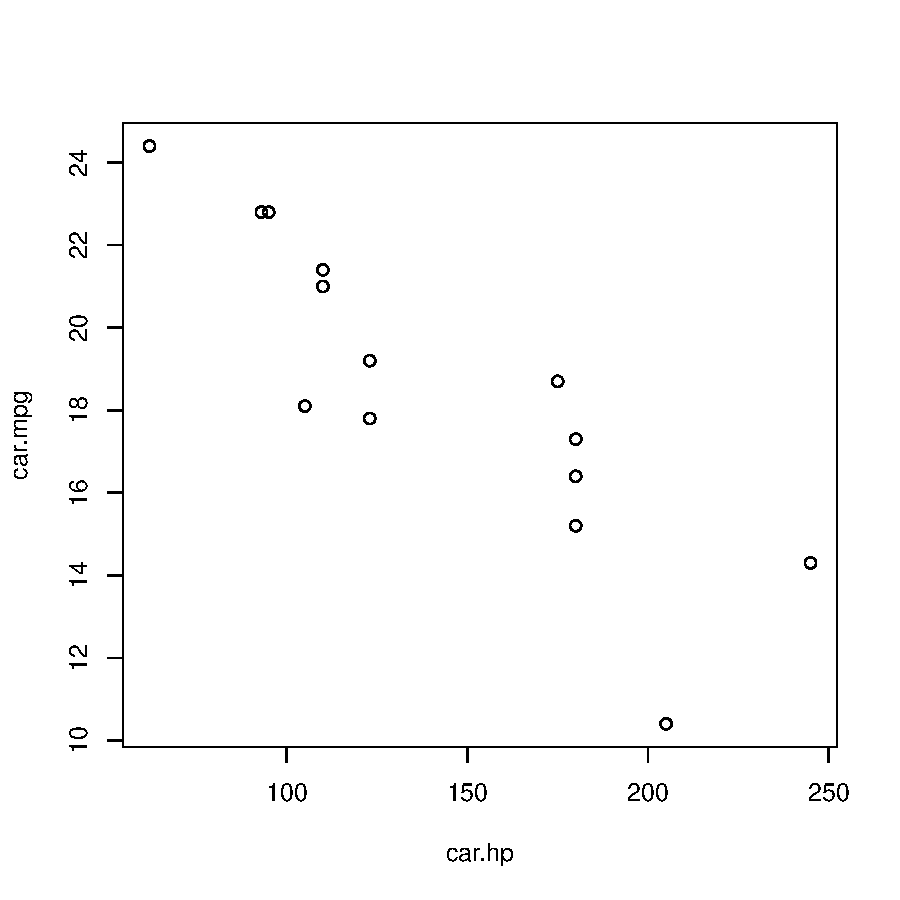
\includegraphics{chapter2-005}
Unsurprisingly as horsepower increases, mpg tends to decrease. We'll investigate this further using simple linear regression in the next section.

\subsection{An initial tour of RStudio}

When you created the \verb+car.hp+ and other vectors in the previous section, you might have noticed the vector name and a short description of its attributes appear in the top right \verb+Global Environment+ window. Similarly, when you called \verb+plot(car.hp,car.mpg)+ the corresponding plot appeared in the lower right \verb+Plots+ window.  

A comprehensive, but overwhelming, cheatsheet for RStudio is available here \url{https://www.rstudio.com/wp-content/uploads/2016/01/rstudio-IDE-cheatsheet.pdf}. As we progress in learning R and RStudio, this cheatsheet will become more useful. For now you might use the cheatsheet to locate the various windows and functions identified in the coming chapters.

%% \subsection{Simple linear regression in R}
%% The \verb+lm()+ function is used to fit linear models in R, including simple linear regression models. Here it is applied to the car data.
%% <<prompt=T>>=
%% car.lm = lm(car.mpg ~ car.hp) ##Fit the model and save it in car.lm
%% summary(car.lm)  ##Basic summary of the model
%% plot(car.hp, car.mpg) ##Scatter plot of the data
%% abline(car.lm) ##Add the fitted regression line to the plot
%% @

\section{How to learn (The most important section in this book!)}
There are several ways to engage with the content of this book and associated learning materials. 

One way is not to engage at all. Leave the book closed on a shelf and do something else with your time. That may or may not be a good life strategy, depending on what else you do with your time, but you won't learn much from the book!

Another way to engage is to read through the book ``passively,'' reading all that's written but not reading the book while at your computer, where you could enter the R commands from the book. With this strategy you'll probably learn more than if you leave the book closed on a shelf, but there are better options.

A third way to engage is to read the book while you're at a computer, and to enter the R commands from the book as you read about them. You'll likely learn more this way.

A fourth strategy is even better. In addition to reading and entering the commands given in the book, you think about what you're doing, and ask yourself questions (which you then go on to answer). For example after working through the example R code above you might ask yourself, ``What would R do if I asked it to calculate the logarithm of a negative number? What would R do if I asked it to calculate the logarithm of a really large number such as one trillion?'' You could explore these questions easily, by just trying things out in the R Console window. 

If your goal is to maximize the time you have to have to binge-watch Stranger Things on Netflix, the first strategy may be optimal. But if your goal is to learn a lot about computational tools for data science, the fourth strategy is probably going to be best.

\section{Getting help}
There are several free (and several not free) ways to get R help when needed. 

Several help-related functions are built into R. If there's a particular R function of interest, such as \verb+log+, \verb+help(log)+ will bring up a help page for that function. In RStudio the help page is displayed, by default, in the \texttt{Help} tab in the lower right window.\footnote{There are ways to change this default behavior.} The function \verb+help.start+ opens a window which allows browsing of the online documentation included with R. To use this, type \verb+help.start()+ in the console window.\footnote{You may wonder about the parentheses after \texttt{help.start}. A user can specify arguments to any R function inside parentheses. For example \texttt{log(10)} asks R to return the logarithm of the argument 10. Even if no arguments are needed, R requires empty parentheses at the end of any function name. In fact if you just type the function name without parentheses, R returns the definition of the function. For simple functions this can be illuminating.} The \verb+help.start+ function also provides several manuals online and can be a quite useful interface to the built in help.

Search engines provide another, sometimes more user-friendly, way to get R questions answered. A Google search often quickly finds something written by another user who had the same (or a similar) question, or an online tutorial that touches on the question. More specialized is \url{rseek.org}, which is a search engine focused specifically on R. Both Google and \url{rseek.org} are valuable tools, often providing more user-friendly information then R's own help system.

R users have written many types of contributed documentation. Some of this documentation is available at \url{http://cran.r-project.org/other-docs.html}. Of course there are also numerous books covering general and specialized R topics available for purchase.

\section{Workspace, working directory, and keeping organized}

The \emph{workspace} is your R session working environment and includes any objects you create. Recall these objects are listed in the \verb+Global Environment+ window. The command \verb+ls()+, which stands for list, will also list all the objects in your workspace (note, this is the same list that is given in the \verb+Global Environment+ window). When you close RStudio, a dialog box will ask you if you want to save an image of the current workspace. If you choose to save your workspace, RStudio saves your session objects and information in a \verb+.RData+ file (the period makes it a hidden file) in your \emph{working directory}. Next time you start R or RStudio it checks if there is a \verb+.RData+ in the working directory, loads it if it exists, and your session continues where you left off. Otherwise R starts with an empty workspace. This leads to the next question---what is a working directory? 

Each R session is associated with a working directory. This is just a directory from which R reads and writes files, e.g., the \verb+.RData+ file, data files you want to analyze, or files you want to save. On Mac when you start RStudio it sets the working directory to your home directory (for me that's \verb+/Users/andy+). If you're on a different operating system, you can check where the default working directory is by typing \verb+getwd()+ in the console. You can change the default working directory under RStudio's \verb+Global Option+ dialog found under the \verb+Tools+ dropdown menu. Once an R session is started in RStudio you can change the working directory using options under the \verb+More+ button under the \verb+Files+ tab in the lower right window. Alternatively, you can set the session's working directory using the \verb+setwd()+ in the console. For example, on Windows \verb+setwd("C:/Users/andy/for375/exercise1")+ will set the working directory to \verb+C:/Users/andy/for375/exercise1+, assuming that file path and directory exist (note, Windows file path uses a backslash, i.e., \verb+\+, but in R the backslash is an escape character, hence specifying file paths in R on Windows uses the forward slash, i.e., \verb+/+). Similarly on Mac you can use \verb+setwd("/Users/andy/for375/exercise1")+. Later on when we start reading and writing data from our R session, it will be very important that you are able to identify your current working directory and change it if needed. We will revisit this in subsequent chapters.

As with all work, keeping organized is the key to efficiency. It is good practice to have a dedicated directory for each R project or exercise. 

%% \begin{vid}{
%%     This video reinforces working directory, workspace, and organization topics. It also covers the {\tt save.image} and {\tt load} functions used to save and load a workspace.}
%% \end{vid}


\section{Quality of R code}

\begin{figure}[htbp]
\includegraphics*[width=5.5in]{chapter2/code_quality.png}
\caption{xkcd: Code Quality}
\label{FIG:COMIC}
\end{figure}

Writing well-organized and well-labeled code allows your code to be more easily read by another person. (See xkcd's take on code quality in Figure \ref{FIG:COMIC}.) More importantly, though, your well-written code is more accessible to you hours, days, or even months later. We are hoping that you can use the code you write in this class in future projects and research.

Google provides style guides for many programming languages. You can find the R style guide \href{here}{https://google.github.io/styleguide/Rguide.xml}. Below are a few of the key points from the guide that we will use right away.


{\setlength{\parindent}{0cm}
\textbf{Naming Files} \\
File names should be meaningful and end in \verb+.R+. If we write a script that analyzes a certain species distribution: \\
GOOD: {\color[RGB]{34,139,34}\verb+african_rhino_distribution.R+} \\
GOOD: {\color[RGB]{34,139,34}\verb+africanRhinoDistribution.R+} \\
BAD: {\color{red}\verb+speciesDist.R+} (too ambiguous)\\
BAD:  {\color{red}\verb+species.dist.R+} (too ambiguous and two periods can confuse operating systems' file type auto-detect)\\
BAD:  {\color{red}\verb+speciesdist.R+} (too ambiguous and confusing)\\

\textbf{Naming Variables} \\
GOOD: {\color[RGB]{34,139,34}\verb+rhino.count+} \\
GOOD: {\color[RGB]{34,139,34}\verb+rhinoCount+} \\
GOOD: {\color[RGB]{34,139,34}\verb+rhino_count+} (We don't mind the underscore and use it quite often, although Google's style guide says it's a no-no for some reason)\\
Bad: {\color{red}\verb+rhinocount+} (confusing)\\

\textbf{Syntax} 
\begin{itemize}
\item Keep code lines under 80 characters long.
\item Indent your code with two spaces. (RStudio does this by default when you press the TAB key.)
\end{itemize}
}

\begin{vid}{
    This video reviews chapter topics and provides additional details on using the RStudio and RStudio Server IDE.}
\end{vid}
